\documentclass{scrartcl}			% defines the kind of document you want to produce

% Include different packages:
\usepackage[utf8]{inputenc}
\usepackage[T1]{fontenc}
\usepackage{lmodern}
\usepackage[english]{babel}
\usepackage{amsmath}
\usepackage{graphicx}           	% include graphics
\usepackage{caption}	
\usepackage{subcaption}	 
\usepackage{hyperref}
\usepackage{epstopdf}
\usepackage{siunitx}
\usepackage{float}

\title{Neuroprothetik Exercise 4 \\ Hodgkin \& Huxley Model}
\author{ Laura Bielenberg }
\date{30. May 2019}

\begin{document} 					% Document begins here

\maketitle
\section{Time constants and steady state values}
Derive the relationship between the rate equations for $\alpha_x$, $\beta_x$ and the time constant $\tau_x$ and steady state value $x_\infty$ with $x \in{m,n,h}$. To gain these two variables bring the gating ODEs found in the appendix A into the following form:
\begin{equation}
\frac{dx}{dt}= \frac{1}{\tau_x}(x_\infty - x)
\end{equation}
\newline
\newline
\textbf{Answer:}
\newline
By rewriting the gating ODEs from appendix A as
\begin{align}
\begin{split}
\frac{dx}{dt} &= [\alpha_x(1-x)-\beta_x x]k\\ &= k(\alpha_x+\beta_x)(\frac{\alpha_x}{\alpha_x+\beta_x}-x)
\end{split}
\end{align}
and comparing this to 
\begin{equation}\label{eq:x_dt}
\frac{dx}{dt} = \frac{1}{\tau_x}(x_\infty-x)
\end{equation}
we find that
\begin{equation}\label{eq:Tau}
\tau_x = [k(\alpha_x + \beta_x)]^{-1}
\end{equation}
and
\begin{equation}\label{eq:x_inf}
x_\infty = \frac{\alpha_x}{\alpha_x+\beta_x}
\end{equation}
for $x \in {m,n,h}$ where $k=3^{0.1(T-6.3)}$.\\
\\
Figure \ref{fig:tx} shows  $\tau_x$  and $x_\infty$ plotted against the voltage $V\in[-100 mV, 100 mV]$ at $\SI{6.3}{\celsius}$ and $\SI{28}{\celsius}$ using the parameters given in the appendix of the exercise sheet.
\newpage
\begin{figure}[H] 
  \begin{subfigure}[b]{0.5\linewidth}
    \centering
    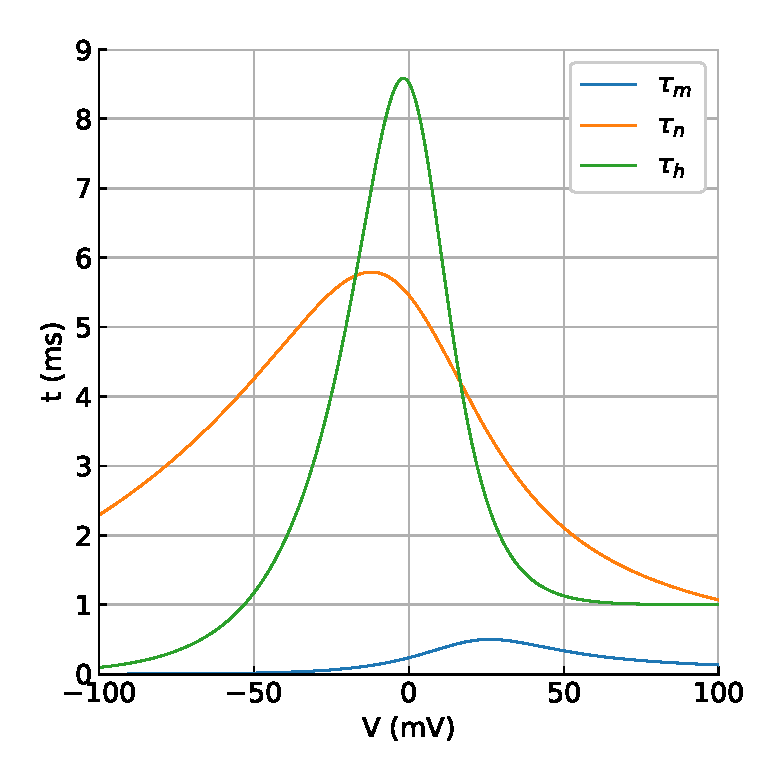
\includegraphics[width=\linewidth]{imgs/timeConst_at_6.eps} 
    \caption{Time constants $\tau_x$ at \SI{6.3}{\celsius}.} 
    \label{fig:tc_63t} 
    \quad
  \end{subfigure}%% 
  \begin{subfigure}[b]{0.5\linewidth}
    \centering
    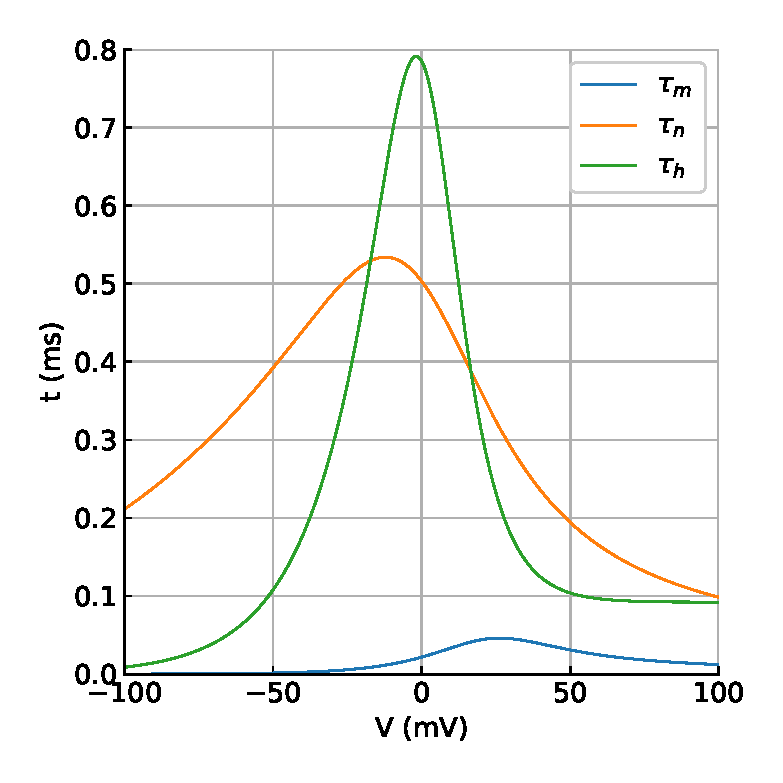
\includegraphics[width=\linewidth]{imgs/timeConst_at_28.eps} 
    \caption{Time constants  $\tau_x$ at \SI{28}{\celsius}.} 
    \label{fig:tc_28} 
    \quad
  \end{subfigure} 
  \begin{subfigure}[b]{0.5\linewidth}
    \centering
    \includegraphics[width=\linewidth]{imgs/x_at_6.eps} 
    \caption{$x_\infty$ at \SI{6.3}{\celsius}.} 
    \label{fig:x_63} 
  \end{subfigure}%%
  \begin{subfigure}[b]{0.5\linewidth}
    \centering
    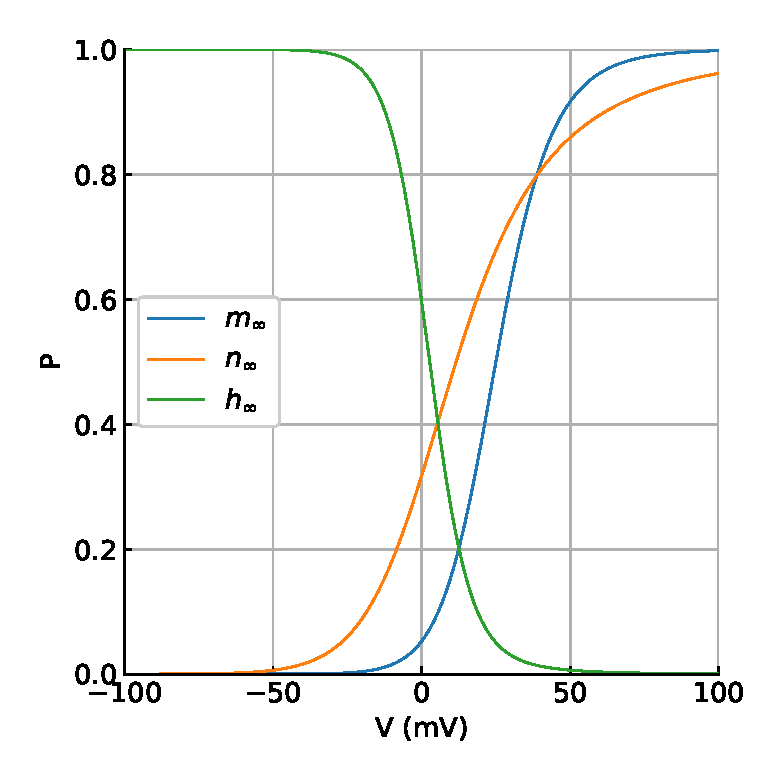
\includegraphics[width=\linewidth]{imgs/x_at_28.eps} 
    \caption{$x_\infty$ at \SI{28}{\celsius}.} 
    \label{fig:x_28} 
    \end{subfigure} 
  \caption{Parameters $\tau$ and $x_\infty$ for the gating variables $m$, $n$ and $h$ for $\SI{6.3}{\celsius}$ and  $\SI{28}{\celsius}$.}
  \label{fig:tx} 
\end{figure}
\newpage
\begin{flushleft}
\textbf{Explanation and interpretation}:\\
\end{flushleft}
Both characteristic values are plottet for $\SI{6.3}{\celsius}$ and $\SI{28}{\celsius}$ respectively and over a membrane voltage range of $V\in[-100\,mV, 100\,mV]$.
Looking at equation~\ref{eq:x_inf} as well as figures~\ref{fig:x_63} and \ref{fig:x_63}, the steady state values show no temperature dependency. The gates timeconstants $\tau_x$ however, are coupled to the temperature by the factor $k$ as can be seen in equation~\ref{eq:Tau} and in figures~\ref{fig:tc_63t} and \ref{fig:tc_28}. While their general behaviour (comparing the shapes of the plots) remains the same, $k$ is used to downscale the timeconstants as the underlying Bolzmann equations would lead to faster processes for higher temperatures.\\
For the steady state gates depicted in figures~\ref{fig:x_63} and \ref{fig:x_28} it can be seen that the open-probability for the activation gates $m$ and $n$ increases increasing membrane potential, while at the same time the open-probability of the inactivation gate $h$ decreases. Also, the slope of the \ce{Na} inactivation gates shows a steaper decline than that of the activation gates showing a higher sensibility to changes in the membrane potential.

\section{Hodgkin \& Huxley Neuron Model}
In contrast to the LIF Model from exercise 3 the Hodgkin \& Huxley Neuron Model will spike on its own due to the nature of the underlying differential equations.
\subsection{Implementation}
See \texttt{hodgkinHuxley.py} for implementation details. The plots are generated by  \texttt{plot\_hh.py}.

\subsection{Experiments}

\begin{figure}[H] 
  \begin{subfigure}[b]{0.5\linewidth}
    \centering
    \includegraphics[width=\linewidth]{imgs/istim_at_6.eps} 
    \caption{Input current at \SI{6.3}{\celsius}.} 
    \label{fig:istim_63} 
  \end{subfigure}%% 
  \quad
  \begin{subfigure}[b]{0.5\linewidth}
    \centering
    \includegraphics[width=\linewidth]{imgs/istim_at_28.eps} 
    \caption{Input current at \SI{28}{\celsius}.} 
    \label{fig:istim_28} 
    \end{subfigure} 
  \caption{Input currents for different temperatures.}
  \label{fig:istim} 
\end{figure}

\begin{figure}[H] 
  \begin{subfigure}[b]{0.5\linewidth}
    \centering
    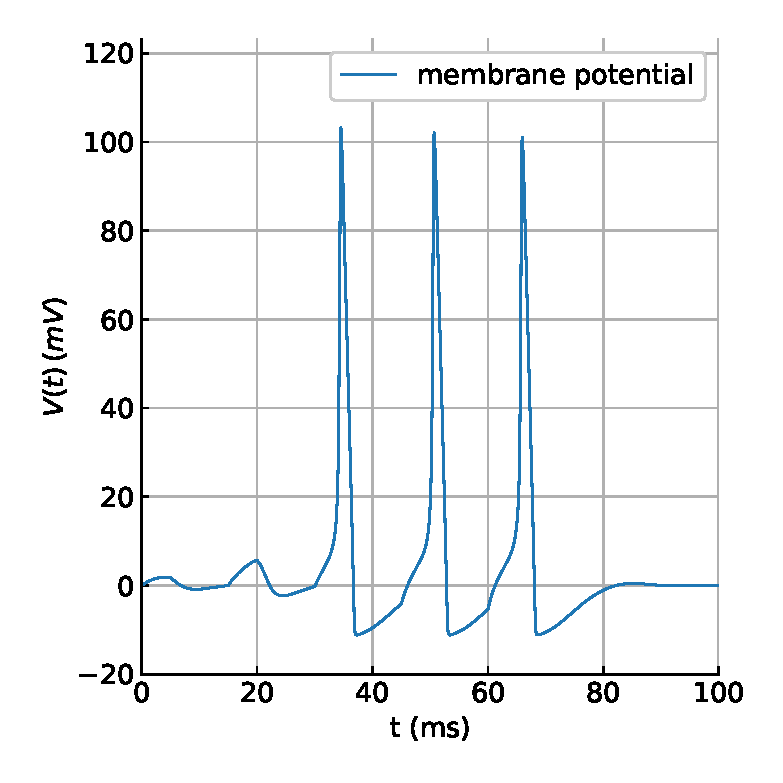
\includegraphics[width=\linewidth]{imgs/membrane_pot_at_6.eps} 
    \caption{Membrane potential for \SI{6.3}{\celsius} and the input visible in figure \ref{fig:istim_63}.} 
    \label{fig:vmem_63} 
  \end{subfigure}%% 
  \quad
  \begin{subfigure}[b]{0.5\linewidth}
    \centering
    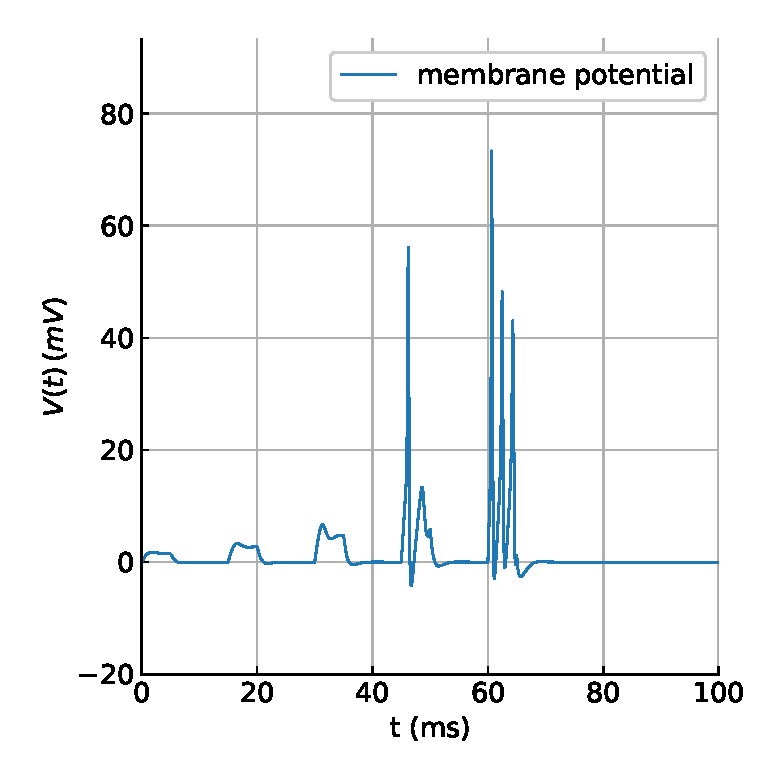
\includegraphics[width=\linewidth]{imgs/membrane_pot_at_28.eps} 
    \caption{Membrane potential for \SI{28}{\celsius} and the input visible in figure \ref{fig:istim_28}.} 
    \label{fig:vmem_28} 
    \end{subfigure} 
  \caption{Membrane potentials for different input current and temperature tuples.}
  \label{fig:vmembrane} 
\end{figure}

\begin{figure}[H] 
  \begin{subfigure}[b]{0.5\linewidth}
    \centering
    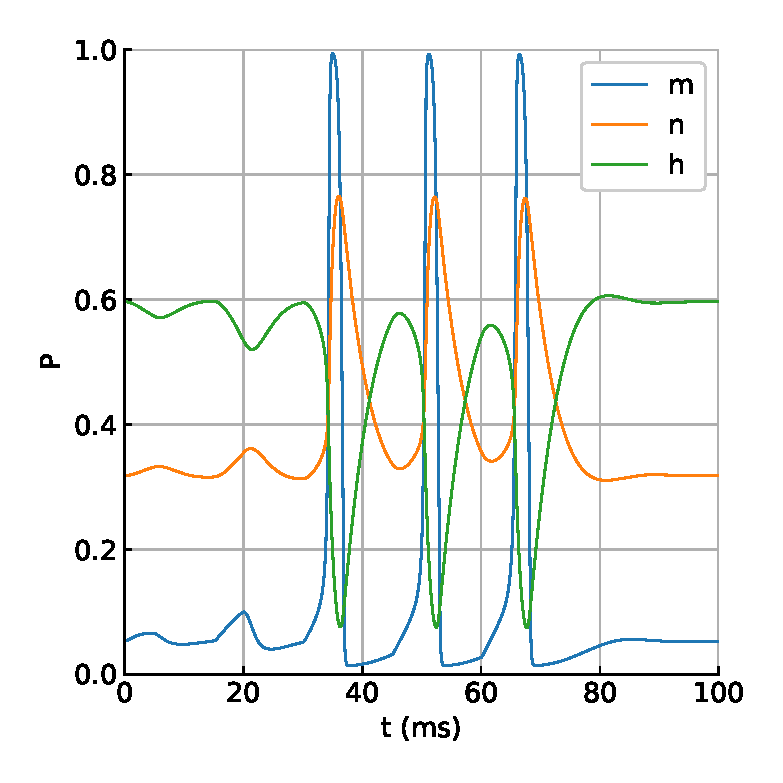
\includegraphics[width=\linewidth]{imgs/gates_at_6.eps} 
    \caption{Gate variables for \SI{6.3}{\celsius} and the input visible in figure \ref{fig:istim_63}.} 
    \label{fig:gates_63} 
  \end{subfigure}%% 
  \quad
  \begin{subfigure}[b]{0.5\linewidth}
    \centering
    \includegraphics[width=\linewidth]{imgs/gates_at_28.eps} 
    \caption{Gate variables for \SI{28}{\celsius} and the input visible in figure \ref{fig:istim_28}.} 
    \label{fig:gates_28} 
    \end{subfigure} 
  \caption{Gating variables m, n, h for different input current and temperature tuples.}
  \label{fig:gates} 
\end{figure}

\begin{figure}[H] 
  \begin{subfigure}[b]{0.5\linewidth}
    \centering
    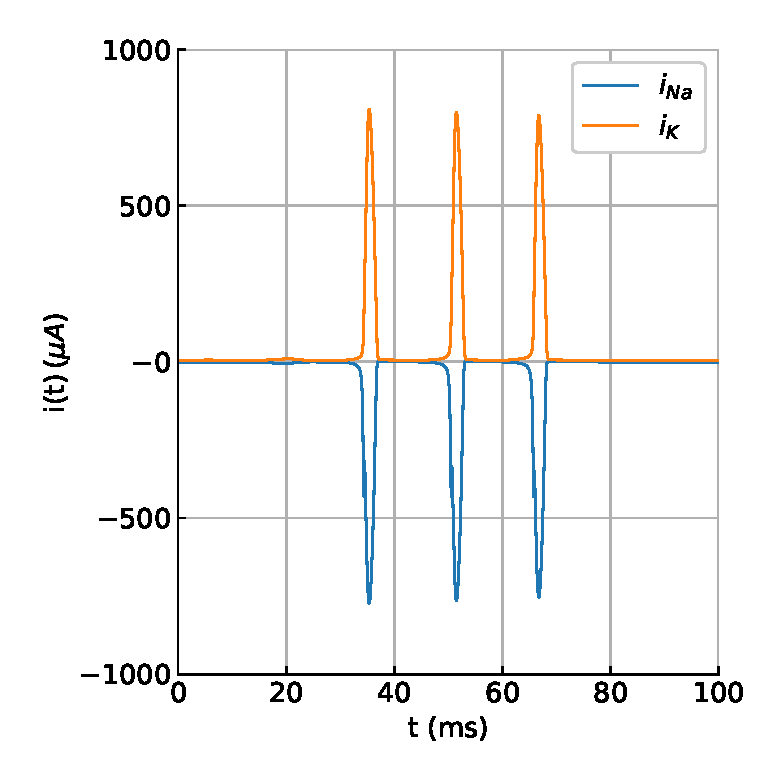
\includegraphics[width=\linewidth]{imgs/ion_currents_at_6.eps} 
    \caption{Currents $i_{Na}$ and $i_{K}$ for \SI{6.3}{\celsius} and the input visible in figure \ref{fig:istim_63}.} 
    \label{fig:curr_63} 
  \end{subfigure}%% 
  \quad
  \begin{subfigure}[b]{0.5\linewidth}
    \centering
    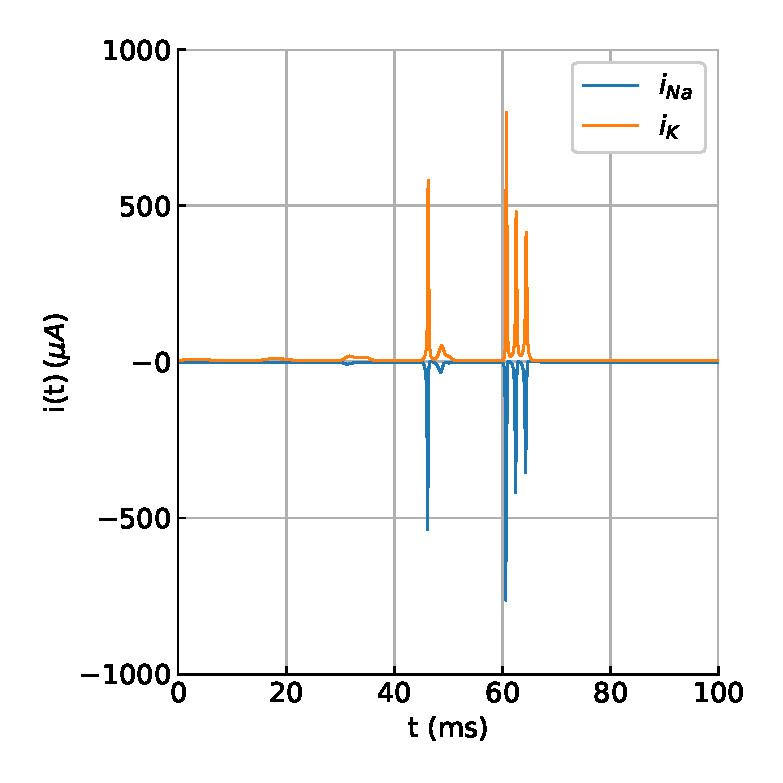
\includegraphics[width=\linewidth]{imgs/ion_currents_at_28.eps} 
    \caption{Currents $i_{Na}$ and $i_{K}$ for \SI{28}{\celsius} and the input visible in figure \ref{fig:istim_28}.} 
    \label{fig:curr_28} 
    \end{subfigure} 
  \caption{Currents $i_{Na}$ and $i_{K}$ for different input current and temperature tuples.}
  \label{fig:curr} 
\end{figure}

\begin{figure}[H] 
  \begin{subfigure}[b]{0.5\linewidth}
    \centering
    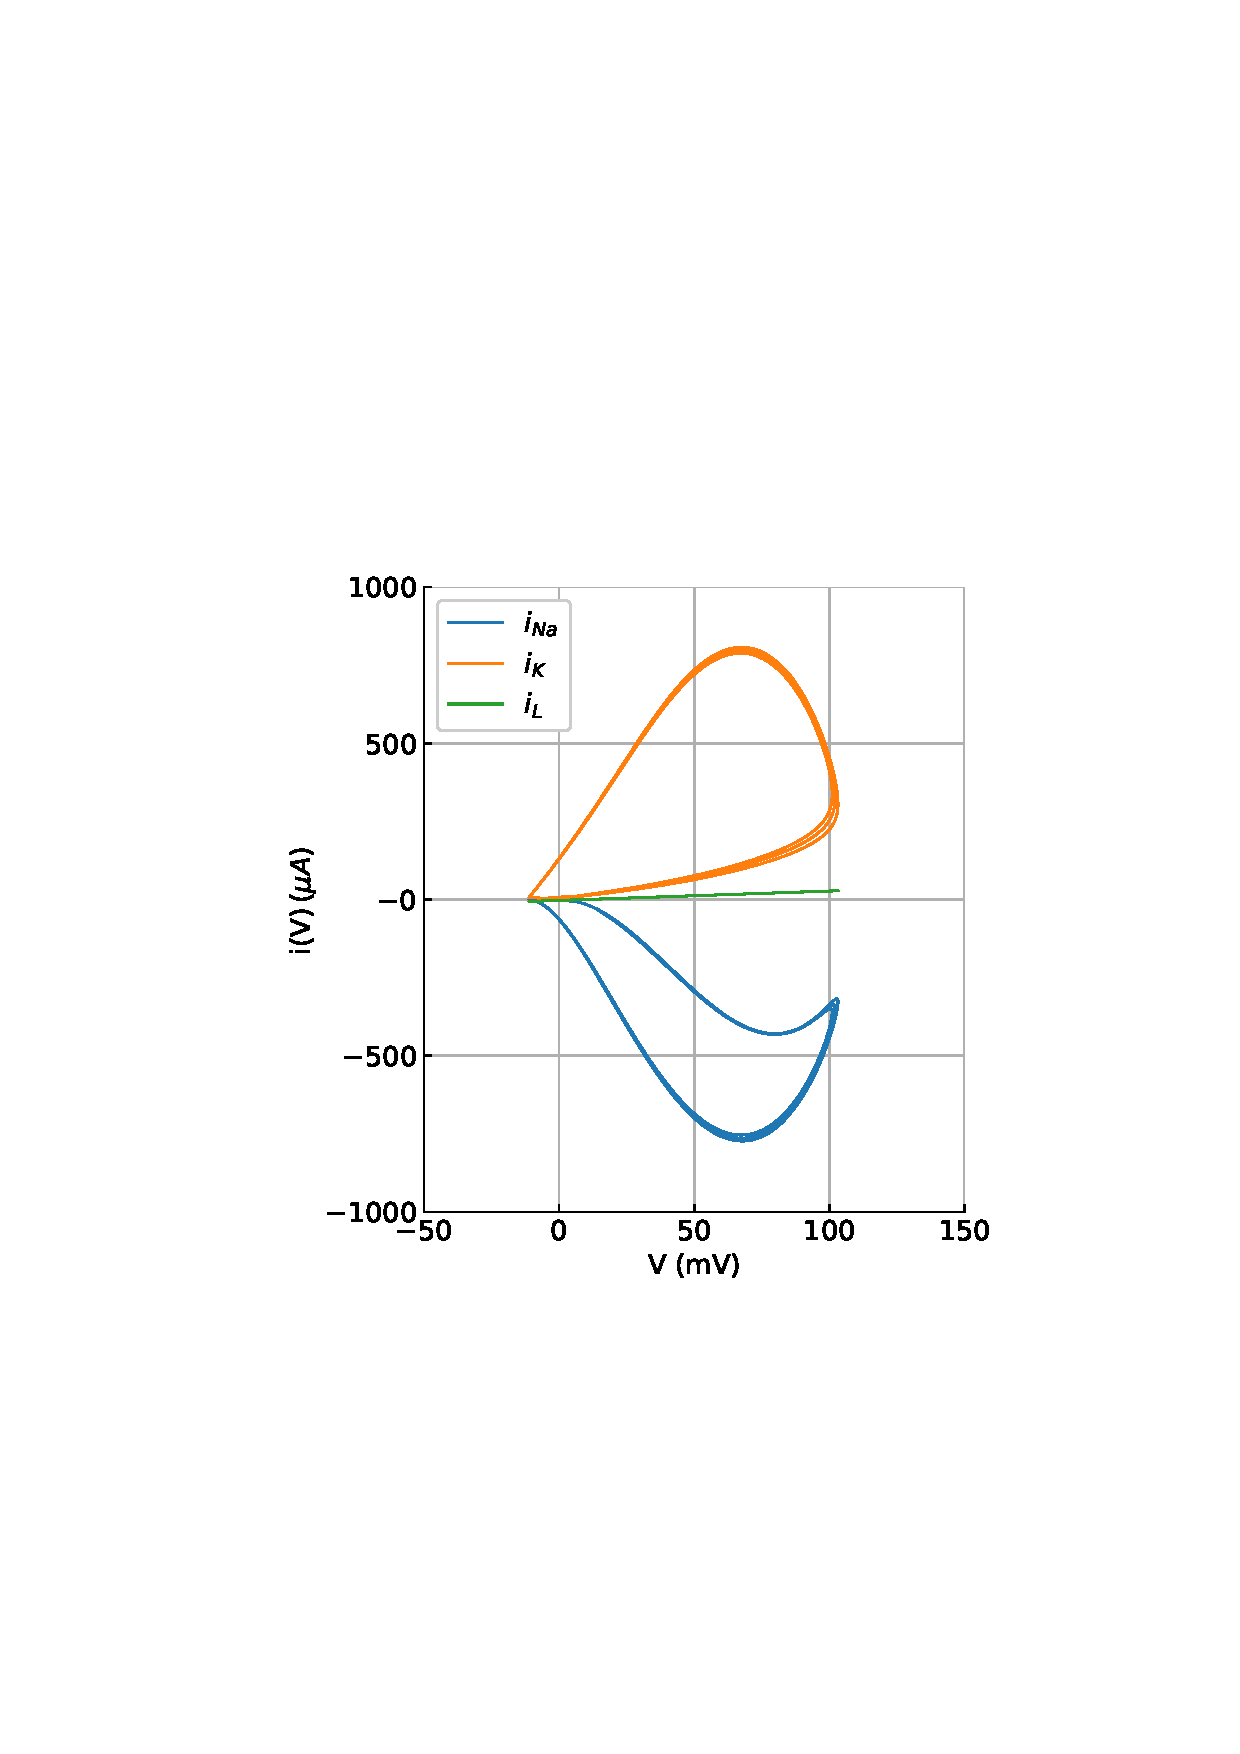
\includegraphics[width=\linewidth]{imgs/current_phases_at_6.jpeg} 
    \caption{Phase plot for \SI{6.3}{\celsius} and the input visible in figure \ref{fig:istim_63}.} 
    \label{fig:phases_63} 
  \end{subfigure}%% 
  \quad
  \begin{subfigure}[b]{0.5\linewidth}
    \centering
    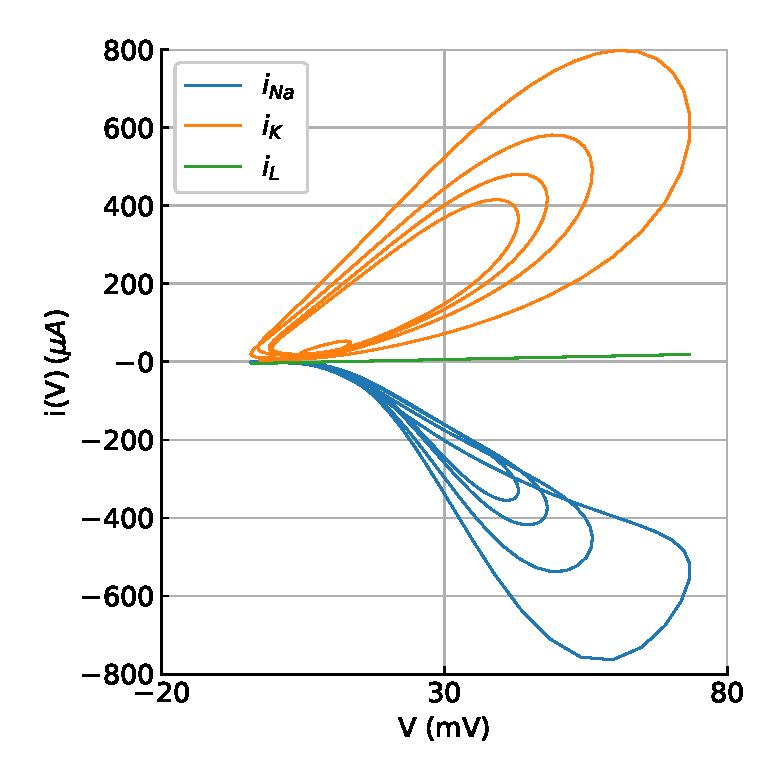
\includegraphics[width=\linewidth]{imgs/current_phases_at_28.eps} 
    \caption{Phase plot for \SI{28}{\celsius} and the input visible in figure \ref{fig:istim_28}.} 
    \label{fig:phases_28} 
    \end{subfigure} 
  \caption{Currents $i_{Na}$ and $i_{K}$ for different input current and temperature tuples.}
  \label{fig:phases} 
\end{figure}

\begin{figure}[H]
    \centering
    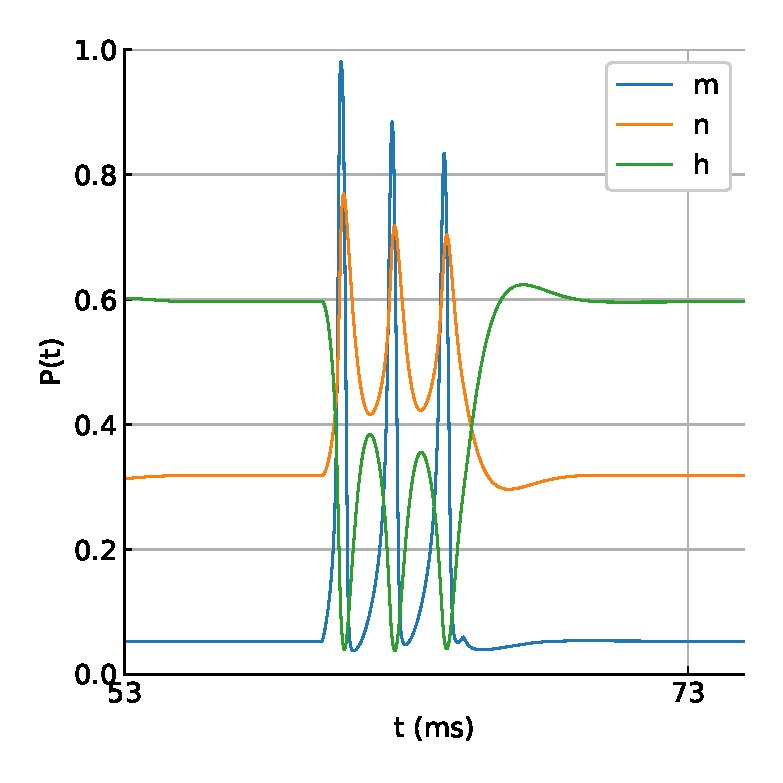
\includegraphics[width=.5\linewidth]{imgs/gates_at_28_from5300.eps} 
    \caption{Close-up of gating variables at $\SI{28}{\celsius}$ from  \ref{fig:gates_28}.} 
    \label{fig:decreasing_peak_explanation} 
\end{figure}

\subsection{Analysis of the results}
In this exercise the HH-model is simulated at two different conditions. Temperatures as well as the stimulus current densities differ between the experiments.
Which means that the different results are can not be allocated to one parameter alone.

\begin{enumerate}
\item \textbf{Describe the difference between the results at $\SI{6.3}{\celsius}$ and $\SI{28}{\celsius}$:}\\

Due to the temperature dependance of the timeconstants given in equation~\ref{eq:Tau}, they are smaller at higher temperatures, which is why the gates react faster to input changes at $\SI{28}{\celsius}$ than at $\SI{6.3}{\celsius}$. The gates dependancy on the timeconstants is also visible in equation~\ref{eq:x_dt}.\\
The stiff behaviour can also be observe by comparing the two plots of the membrane potential in figure~\ref{fig:vmembrane}.
The steps of the input current are filtered at $\SI{6.3}{\celsius}$ and the system converges slower than at higher temperatures, due to the low-pass behaviour of the system. The membrane potential at $\SI{6.3}{\celsius}$ on the other hand looks more spiky.\\
Furthermore, exitation with $\SI{32}{\micro\ampere}$ at $\SI{28}{\celsius}$ leads to a fast sequence of cell excitations with decreasing peak amplitude, due to missing refractory time between the excitations. 

\item \textbf{How is the action potential generated and what is the role of the different currents and gating variables:}\\

There are three different gating variables considered in the HH-model. The sodium and potassium channel activation gates, m and n respectively, and the sodium channels inactivation gate h. Each sodium channel consists of three m gates responsible for opening the channel and one h gate which is supposer to inactivate the channel. The potassium channels on the other hand are build from four n gates.\\ The main currents involved in de- and repolarisation of the membrane potentials are $i_{Na}$ and $i_{K}$.\\
For an action potential to be generated the cell membrane potential has to increase beyond a certain threshold value $V_{thr}$. Once $V_{thr}$ is surpassed the m and n gates are activated and the fast sodiums channels open, enabling more sodium to flow into the cell. This opening od sodium channels in return further depolarises the cell membrane (positive feedback) opening up more and more sodium channels while $V_m$ approaches the sodium Nerst potential. At the same time potassium channels start to open and the inactivation gates begin close some of the sodium channels (both are much slower than the sodium activation gates). The peek is reached when the potassium efflux $i_{K}$ overtakes the sodium influx $i_{Na}$. Now the cell starts to repolarize. The inactivation gates close more and more sodium channels while the flow through the potassium channels pushes the membranepotential continuously towards the potassium Nernst potential. Since those channels are slow to close, the cell is hyperpolarised before reaching its resting potential at which all voltage dependent channels are back in their steady states.
  
\item \textbf{Explain why consecutive action potentials decrease in amplitude (at $\SI{28}{\celsius}$):}\\

The membrane potential in Figure~\ref{fig:vmem_28} shows a pattern of consecutive action potentials with decreasing amplitudes between $t=\SI{60}{\milli\second}$ and $t=\SI{65}{\milli\second}$. This can be explained by having a closer look at the gating variables during that timespan, depicted in Figure~\ref{fig:decreasing_peak_explanation}.
While in the first experiment at $6.3^\circ C$ the neuron can passively recover from the action potential by restoring the membranes resting potential and steady state this is not possible in the second experiment at $28^\circ C$ coupled with an input current of $\SI{32}{\mu A}$.
The closeup plot of the activation gates shows that the gates have not yet had the chance to get back to their steady values before the next cell depolarisation is started.
It can be seen, that the open-probability for the sodium inactivation gate is only at $h=\frac{h_{rest}}{2}$ to $\frac{h_{rest}}{3}$, leaving more sodium channels inactivated and thus decreasing the possible sodium ion influx. This becomes clear also when looking at the reduce ionic currents in Figure~\ref{fig:curr_28}. Due to this circumstance the rise of membrane potential is in over all slower.

\item \textbf{How can you interpret the phase plot:}\\

The first observation, looking at both phase plots in Figure~\ref{fig:phases} is, that the leakage current $i_{leak}$ appeares to be a staight line, depending linearly on the membrane potential and barely changing on the intervall of $\SI{0}{\milli\volt}$ to $\SI{100}{\milli\volt}$.\\
Figure~\ref{fig:phases_63} shows the phase plot for $\SI{6.3}{\celsius}$. The arrows show the direction of the $i_{Na}$ and $i_{K}$ phase diagrams over time: clockwise for sodium, counterclockwise for potassium.\\ It can be seen that in the beginning of the depolarisation up to $\SI{10}{mV}$ both sodium and potassium current are around $0$. As the depolarisation increases, the voltage depend sodium and potassium channels are activated. Since the sodium channels timeconstant $\tau_m$ is much faster than the potassium channels, we observe a steep increase in sodium current while the potassium current increases almost only linearly. As the increased influx of sodium further depolarises the membrane towards the sodium equilibrium voltage, more and more voltage dependant sodium channels open, leading to a steady increase in sodium inflow (positive feedback).\\ At around $\SI{80}{\milli\volt}$ $i_{Na}$ reaches a local maximum. Now the slower inactivation gate $h$ starts inactivating parts of the sodium channels, and $i_{Na}$ starts to decrease. When the membrane potential reaches about $\SI{100}{\milli\volt}$ the action potassium reaches it's peek.\\ Though both $i_{Na}$ and $i_{K}$ increase, the potassium efflux starts overtaking the inward sodium current, which leads to the decrease of the cells membrane potential. While $V_m$ decreases the sodium and potassium gates close. Again, the sodium gates are faster. The continuing potassium efflux leads to a short hyperpolarisation. Once all voltage gated channels are back in their initial state the membrane potential goes back to $V_{rest}=0$.

\item \textbf{Explain the difference between the LIF and the HH model, why would you implement one or the other:}\\

The  leaky integrate and fire neuron model is a theoretical neuron model that can be seen as a functional approximation of the Hodgkin & Huxley model which yields a passive description of the cell membrane potential based on a simplified circuit consisting of a resistor, a capacitoy and a battery. It is commonly used in computational investigations of spiking neurons. However, action potentials need to be introduced by hand by defining a Voltage $V_{spike}$ to be triggered when the membrane potential surpasses a predefined threshold $V_{thr}$ and hyperpolarisation is neglected. Over all, the LIF model shows of the basic idea behind action potentials, but does not in fact model the actual behaviour observed in nature.  
\newline
In contrast to that, the Hodgkin \& Huxley model is based on actual experiments on the giant axon of the squid.
The HH-model takes in to account not only the leakage conductivity, membrane voltage, capacity and battery but models the complete cell dynamics down to the single ion-channels and gating variables by using a single set of four differential equations. Those describe the cell dynamics in the resting as well as the action potential and repolatisation phase. 
\end{enumerate}
\end{document}